\documentclass{article}
\usepackage{graphicx}

%Used for systems of equations
\usepackage[overload]{empheq}
\usepackage[inline, shortlabels]{enumitem}

%Used for aligning graphics so they don't go flying of
\usepackage{float}

%Used for automatically referencing figures
\usepackage{nameref}

\title{Analyzing melanotaeniidae and osphronemidae population interaction models with computational 
and analytical solutions of ordinary differential equations}
\author{Emil Svenberg}
\date{2020-04-30}


\begin{document}
\maketitle
\begin{center}
    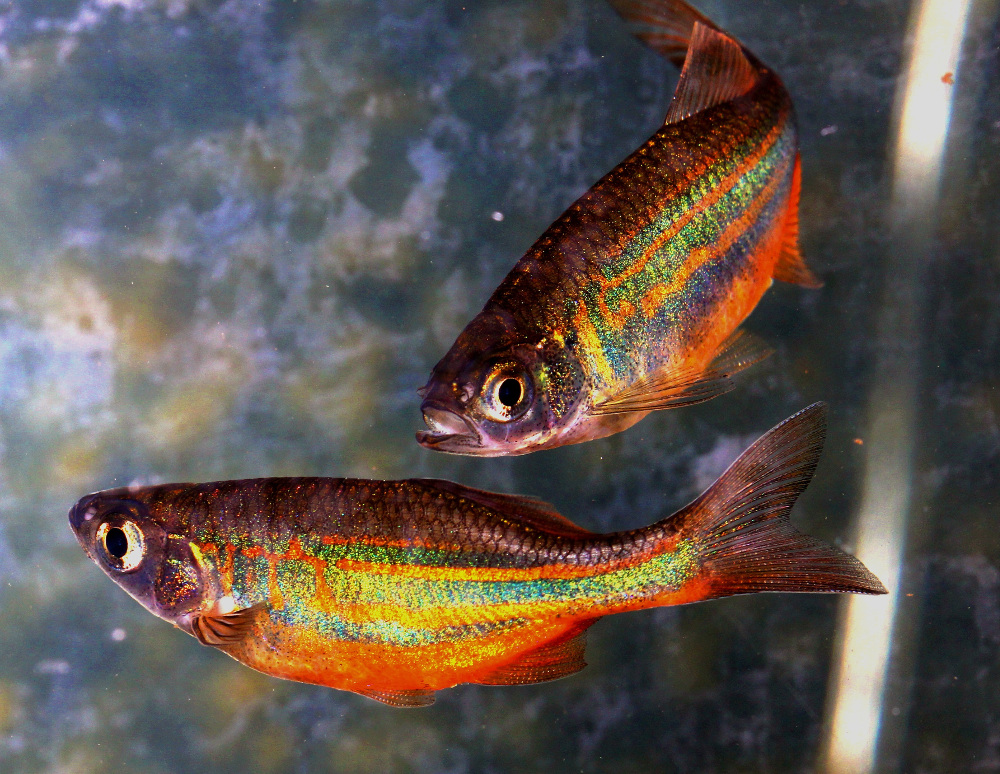
\includegraphics[scale=0.3]{../figures/rainbowfish.jpg}
\end{center}
\pagebreak
\tableofcontents
\pagebreak
\section*{Summary}
\addcontentsline{toc}{section}{Summary}
\begin{flushleft}
    An analysis of a fish population at a popular aquarium for a shop owner was
    shown to be necessary. The shop owner wanted both rainbowfish and
    gouramis, despite gouramis appetite for rainbowfish so we
    needed to build a mathematical model to see if the populations
    would stabilize at an equilibrium or if they would die off over time.

\end{flushleft}

\begin{flushleft}
    A system of differential equations were used to model the fish populations
    in Python using euler's formula. It was then shown
    that an equilibrium does in fact exist.
\end{flushleft}

\begin{flushleft}
    The conclusion is that the aquarium owners original idea
    does in fact work, and that the fishes
    form a stable equilibrium at roughly 31 rainbowfish and 12 gourami. This shows
    that having both fishes in the same aquarium is feasible. However the modell
    cannot control for unexpected occurrences.
\end{flushleft}
\addcontentsline{toc}{section}{List of Variables}
\section*{List of Variables}

\begin{itemize}
    \item[t:] Time in days
    \item[P(t):] Population of rainbowfish at time t
    \item[G(t):] Population of rainbowfish at time t
    \item[a:] rate at which rainbowfish reproduce (0.7)
    \item[b:] rate at which rainbowfish are sold (20)
\end{itemize}
\section{Introduction}
\begin{flushleft}
    The Melings Lake in Fagersta, Västmanland, Sweden has been without
    fish for a hundred years. Today conservationists has asked us if
    an reintroduction of fish could boost the ecosystem. We decided on
    two types of fish and what the potential outcome would be. Would these
    two fishes go extingt and eat eachother up, or would they live in equelibrium?

\end{flushleft}

\begin{flushleft}
    Since you can only buy so many fish we need to know how many is feasable
    and if the population will stabilize at a good point that doesn't
    lead to bad consequences.

\end{flushleft}

\begin{flushleft}
    The purpose of this research is to find out how the fish will behave
    and if they will live in equilibrium with nature so that this effort
    is worth while.
\end{flushleft}

\begin{flushleft}
    The limitations of this project is that it cannot simulate all of nature.
    It also doesn't take into account
\end{flushleft}

\begin{flushleft}
    Outline for the report
\end{flushleft}
% Several core chapters
\section{First Model}

\subsection{Deriving the ODE for the rainbowfish population}

\begin{flushleft}
    An Ordinary Differential Equation needs to model the rainbow fish population change.
    The growth rate of the rainbowfish population is 70\% with
    a maximum aquarium capacity of 750 fishes. The death rate is
    estimated to be 0.001 because one fish lives for 1000
    days, therefore the odds of a fish dying is 0.001, which is then
    multiplied by the number of fishes. $0.001P(t)$
    However this is negligible and is
    removed since the decrease it makes is really small.
    However, 20 rainbowfishes are sold every day,
    so that's included in the model and is not negligible.
\end{flushleft}

\begin{equation}
    \frac{dP}{dt} = 0.7P(t)(1-\frac{P(t)}{750})-20
\end{equation}

\subsection{Results from numerical solution in Python}
\begin{flushleft}

    The model was then solved numerically in Python using
    euler's formula with timestep $\Delta t=\frac{1}{16}$
    which gave the following results:

\end{flushleft}

\begin{figure}[H]
    \centering
    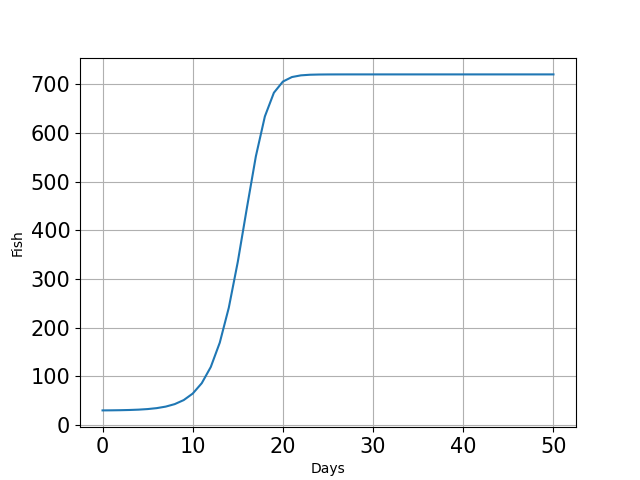
\includegraphics[scale=0.4]{../figures/Figure_1.png}
    \caption{The number of rainbowfish over time with $P(0)=20$}
\end{figure}

\begin{flushleft}
    As we can see, the amount of rainbowfish approaches somewhere
    above 700.
    The exact amount is 720.2, but since you can not have
    fractional fish we can approximate it to 720. This is
    a stable equilibrium point as the population would decrease if it went up and increase if it was lowered.
\end{flushleft}

\begin{flushleft}
    As a conclusion this model does work for one fish,
    however we want to introduce a second type of fish
    into the model. The gourami.
\end{flushleft}


\section{Model including the second fish}

\begin{flushleft}
    The fishowner desperately wanted two types of competing fish species:
    rainbowfish and gourami. The budget was for 20 rainbowfish and 5 gourami.
    To make sure that both fishes both had enough food and didn't manage to kill eachother
    we made a system of differential equations. In this case they interact with each other.
    There is a 4\% chance that a gourami will kill a rainbowfish, thus the $-0.04PG$.
    Gouramis also don't survive on their own so they slowly die, explaining the $-0.25G$
\end{flushleft}

\begin{align*}[left = \empheqlbrace]
    \frac{dP}{dt}= 0.7P-0.007P^2-0.04PG \\
    \frac{dG}{dt} = -0.25G+0.008PG
\end{align*}

\begin{flushleft}
    Now doing the rest was easy. So easy in fact that I wanted to shoot my foot
    with a rocket launcher. The result was the following:

\end{flushleft}
\begin{center}
    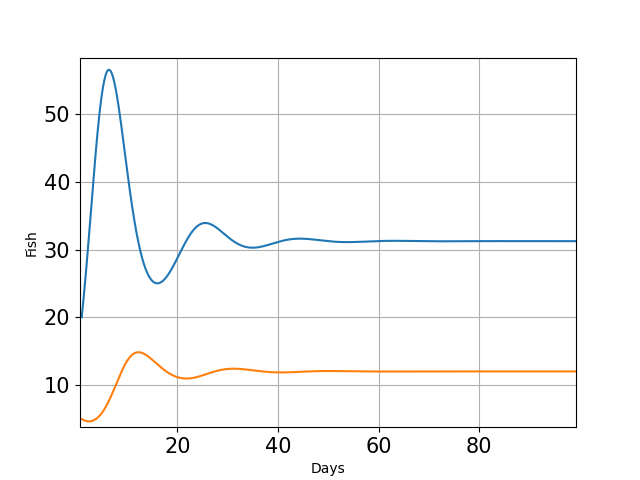
\includegraphics[scale=0.5]{../figures/Figure_2.png}
    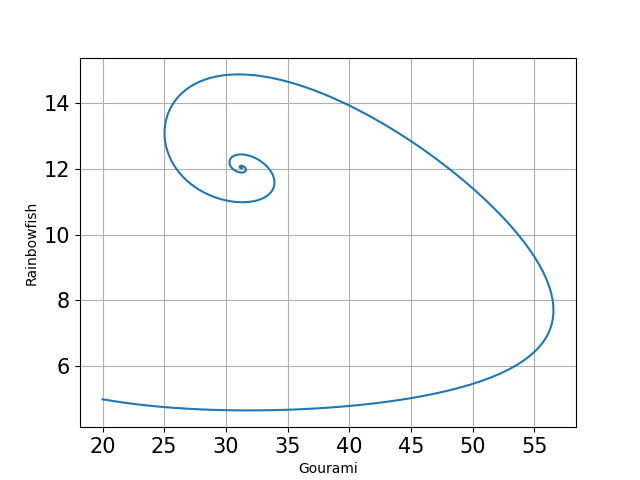
\includegraphics[scale=0.5]{../figures/Figure_3.png}

\end{center}

\begin{flushleft}
    These models tells us that the fish seem to approach an equilibrium at roughtly
    30 rainbowfishes and 12 gourami. Modelling a few more scenarios with different
    starting populations reveal that there is a stable equilibrium point aslong as
    the amount of fish of one species is more than 0.

\end{flushleft}

\begin{center}
    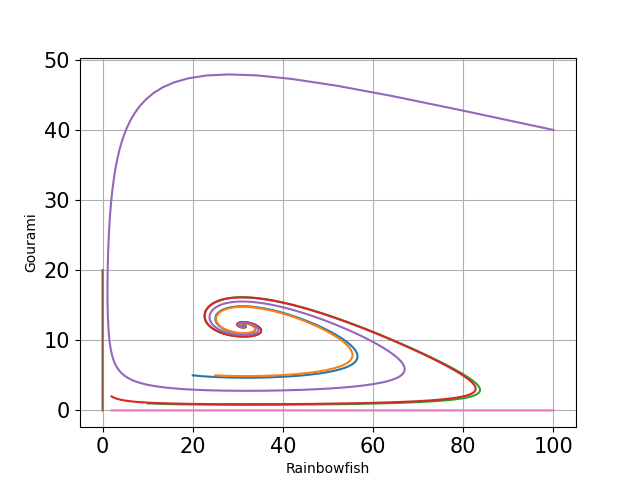
\includegraphics[scale=0.5]{../figures/Figure_4.png}

\end{center}
\section{Conclusions}
\begin{flushleft}
    Could we keep 20 rainbowfish and 5 gouramis?
    Indeed this is the case. With our desired starting population of
    20 rainbowfish and 5 gouramis the fish population reaches a stable equilibrium.
    And this equilibrium is reached even with a large range of starting populations.
    This also implies the possibility of buying fewer fishes to save money.
\end{flushleft}

\begin{flushleft}
    However this model can only explain so much. Birth rates and death
    rates may be affected by unknown causes. And it cannot model the fact
    that fishes lay and hatch many eggs at once instead of continuously over time.
    But despite these drawbacks it's safe to say that the fishes will reach a stable
    equilibrium point.
\end{flushleft}
%\section{Appendix}

\end{document}